\documentclass[a4,paper,fleqn]{article}

\usepackage{layout}

\title{AES - Übung 3}
\date{10. März 2016}
\author{Markus Birrer \\
        Yannick Inderbitzin\\
        Daniel Winz}

\begin{document}
\maketitle
%\clearpage
\vfill
\tableofcontents
\vfill
\clearpage

\section{Kurzfragen}
\begin{itemize}
\item Wie ist die Energie- und Leistungsdichte eines SCAPs definiert? \\
    \[ E' = \frac{1}{2 \cdot m} \cdot C \cdot {U_{SCAP_{max}}}^{2} \]
    \[ P' = \frac{U_{SCAP_{max}} \cdot I}{m} 
    = \frac{U_{SCAP{_{max}}}}{\left(R_{S} + R_{L}\right) \cdot m} 
    \cdot \frac{U_{SCAP_{max}}}{2} 
    = \frac{{U_{SCAP_{max}}}^{2}}{4 \cdot R_{S} \cdot m} \]
\item Wie gross ist eine SCAP-Zeitkonstante typisch? Was last sich davon 
ableiten? \\
    Im Bereich von $1\si{\second}$ ($\tau = R_{i} \cdot C$)
\item Was lässt sich über den Wirkungsgrad von SCAPs generell aussagen? Wie 
gross ist er bezogen auf die Leistung, die durch die 
Leistungsdichte-Definition gegeben ist. Kommentar? \\
    Wirkungsgrad: 0.85 \ldots 0.98 \\
    Die Leistungsdichte ist sehr hoch, die Energiedichte hingegen ist gering. \\
    Bei starker Belastung (Lade-/Entladezeit) sinkt der Wirkungsgrad massiv 
    (0-0.5) \\
\item Wann macht die Kombination von Supercaps und Batterien Sinn? Was gilt es 
bei der Kombination von Supercaps und Batterien zu beachten? \\
    Die Kombination von Batterie und Supercap macht Sinn, wenn sowohl während 
    langer Zeit Leistung benötigt wird (Energie = Akku) und gleichzeitig 
    starke Schwankungen in der Leistung vorhanden sind (Leistung = Supercap)
\item Gibt es Unterschiede bei der Integration von Supercaps gegenüber 
Batterien? \\
    Ja, Supercaps verhalten sich anders als Batterien, u.a. Leistungsdichte 
    und Entladung. Dies muss bei der Integration in Betracht gezogen werden. 
    z.B. dickere Leitungen für Supercaps oder auch ein anderes, angepasstes 
    Energiemanagement-System. Auch der Ausgleich der Zellen muss im Auge 
    behalten werden.
\end{itemize}

\section{Berechnung LiIonen Batterien als Vergleich}
\begin{itemize}
\item Berechnen Sie die Energiedichte. \\
    $80\si{\watt\hour/per/killogram}$ \\
    pro Zelle zu 365\si{\gram} = 29.2\si{\watt\hour\per Zelle}
\item Berechnen Sie die Leistungsdichte der Ladung und der Entladung. 
Kommentare? \\
    \[ P = \frac{U \cdot I}{m} \]
    Ladung: 
    \[ \frac{3.2\si{\volt} \cdot 30\si{\ampere}}{0.365\si{\kilogram}} = 263 \si{\watt\per\kilogram} \]
    Entladung: 
    \[ \frac{3.2\si{\volt} \cdot 100\si{\ampere}}{0.365\si{\kilogram}} = 876.7 \si{\watt\per\kilogram} \]
\item  Berechnen Sie den Wirkungsgrad für nur eine 10C Entladung und separat 
nur für eine 3C Ladung.  Berechnen Sie den Gesamtwirkungsgrad für den 
gesamten Zyklus (Entladung und Ladung).  Annahme: Nur CC Ladeverfahren für 
den ganzen Energieinhalt. \\
    Wirkungsgrad für 10C Entladung $\to$ 100\si{\ampere}: 
    \[ R_{tot} = \frac{U}{I} = \frac{3.2\si{\volt}}{100\si{\ampere}} 
    = 0.032\si{\ohm} \]
    \[ R_s = 0.005\si{\ohm} \Rightarrow R_L 
    = R_{tot} - R_S = 0.032\si{\ohm} - 0.005\si{\ohm} = 0.027\si{\ohm} \]
    \[ \eta_1 = \frac{R_L}{R_L + R_S} = \frac{0.027}{0.032} = 0.843 \]
    Wirkungsgrad für 3C Ladung $\to$ 30\si{\ampere}: 
    \[ R_{tot} = \frac{U}{I} = \frac{3.65\si{\volt}}{30\si{\ampere}} 
    = 0.121\si{\ohm} \]
    \[ R_s = 0.005\si{\ohm} \Rightarrow R_L 
    = R_{tot} - R_S = 0.121\si{\ohm} - 0.005\si{\ohm} = 0.116\si{\ohm} \]
    \[ \eta_2 = \frac{R_L}{R_L + R_S} = \frac{0.116}{0.121} = 0.958 \]
    Gesamtwirkungsgrad für gesamten Zyklus (Entladung und Ladung) nur CC: \\
    \[ \eta_{tot} = \eta_1 \cdot \eta_2 = 0.843 \cdot 0.958 
    = 0.808 \Rightarrow 80.8\% \]
\end{itemize}

\section{Messung Supercaps}
\subsection{Bestimmung Innenwiderstand}
Zunächst wird der SCAP auf eine Spannung von 2.7\si{\volt} aufgeladen. Dazu 
wird beim ein maximaler Strom von 30\si{\ampere} eingestellt. Die Ladung 
erfolgt zunächst als Konstantstromladung (CC). Nach dem Erreichen der 
Ladeschlussspannung wird der Ladevorgang als Konstantspannungsladung (CV) 
fortgesetzt. 

\begin{figure}[h!]
    \centering
    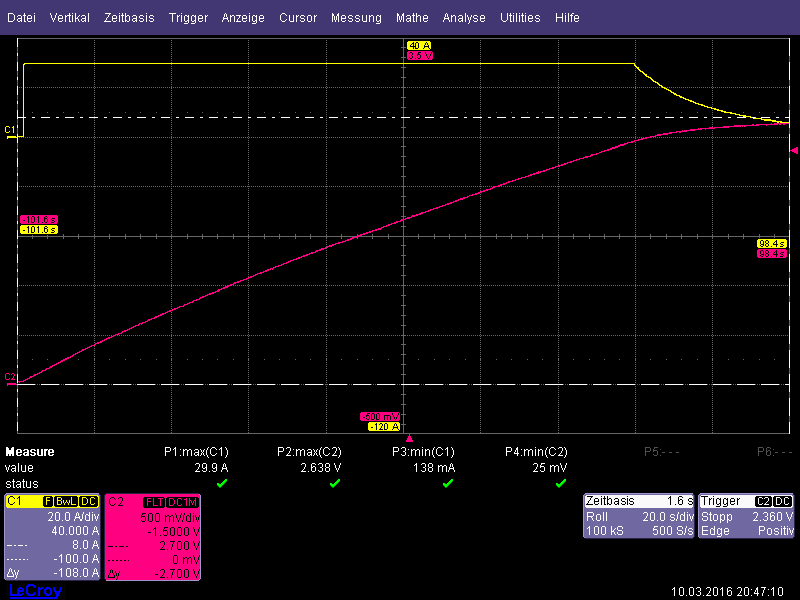
\includegraphics[width=1.0\textwidth, trim=0 20 0 45, clip=true]{fig/charge.png}
    \caption{Ladevorgang $\to$ 30\si{\ampere}}
    \label{fig:charge}
\end{figure}

\noindent
Anschliessend wird der SCAP zur Bestimmung des Innenwiderstandes mit einem 
Strom vom 100\si{\ampere} entladen. Dabei wird die Spannung des SCAP gemessen. 
Aus dem Spannungsabfall nach dem Einschalten der Last kann der Innenwiderstand 
berechnet werden. 

\begin{figure}[h!]
    \centering
    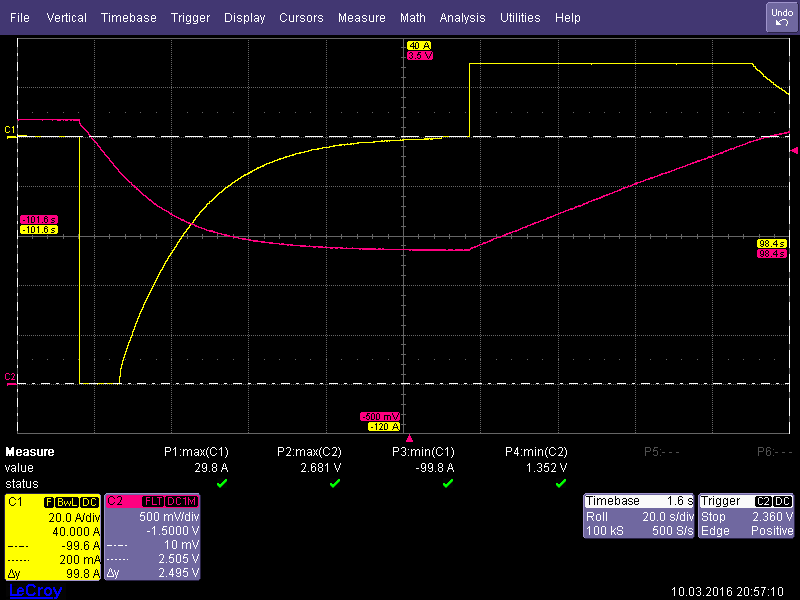
\includegraphics[width=1.0\textwidth, trim=0 20 0 45, clip=true]{fig/discharge2.png}
    \caption{Endladevorgang $\to$ 100 \si{\ampere}}
    \label{fig:discharge_i}
\end{figure}

\begin{figure}[h!]
    \centering
    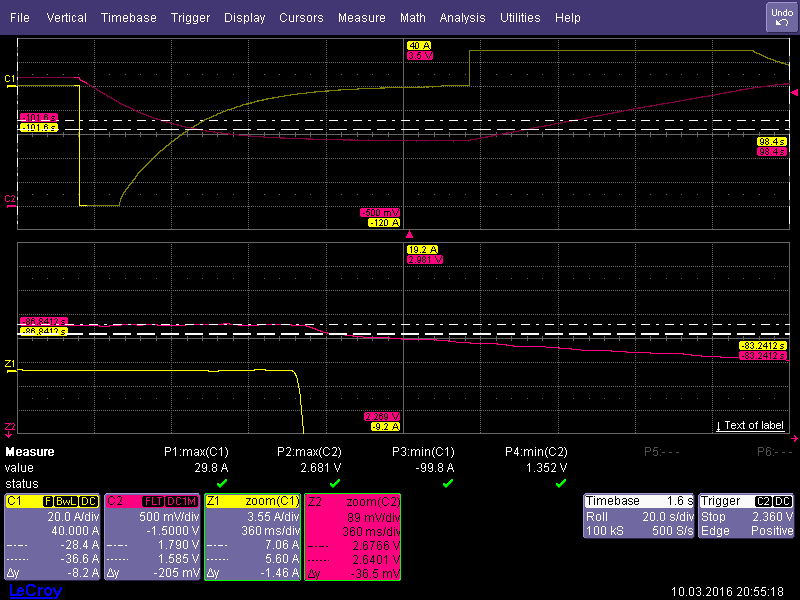
\includegraphics[width=1.0\textwidth, trim=0 20 0 45, clip=true]{fig/discharge1.png}
    \caption{Spannungsverlauf zu Begin des Endladevorgangs}
    \label{fig:discharge_u}
\end{figure}

\noindent
Mit einem Kurzschlussversuch \ldots

\begin{figure}[h!]
    \centering
    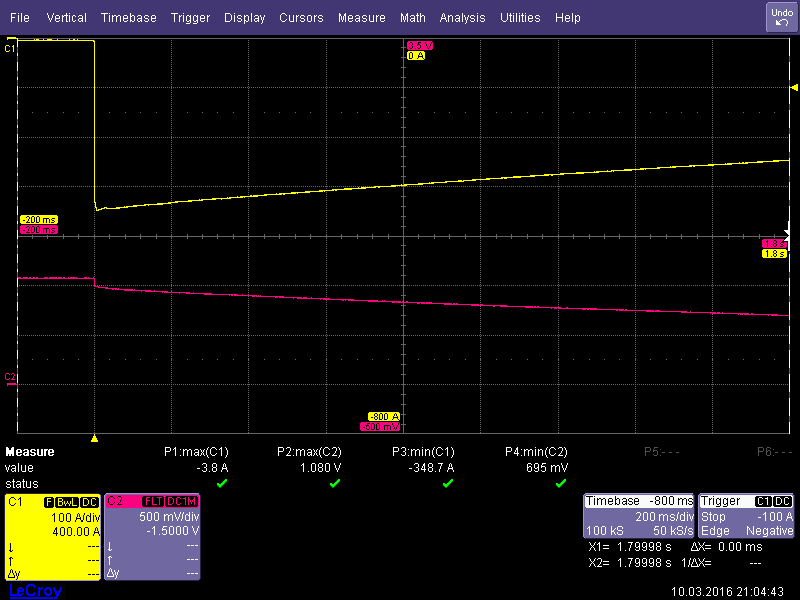
\includegraphics[width=1.0\textwidth, trim=0 20 0 45, clip=true]{fig/short.png}
    \caption{Kurzschlussversuch}
    \label{fig:short}
\end{figure}

\subsection{Messung Kurzschluss}
\subsection{Schlussdiskussion}

\section{Bewertungsbeispiel Akkubohrer}

\end{document}
